\chapter{Simulation study}
\label{chap:simulation_study} 
\section{Data generating process}
To evaluate the finte sample performance of the two proposed method, 
we conduct a simulation study based on the DGP taken 
from Section 5.1 of \citeA{blackwellEffectPoliticalAdvertising2024}. 
In this 
DGP, the scenario which we simulate is a study design 
where individuals are exposed to a binary treatment
(e.g., receiving a political advertisement) over a period 
fixed period of time, and the outcome of interest
is measured only once at the end of the study period 
(e.g., voting behavior). The treatment assignment
is influenced by both observed covariates and an 
unmeasured time-invariant confounder (e.g., political
leaning). The outcome is affected by the treatment 
received at the final time point, the cumulative 
effect of treatments received in the last three time points, 
the mean of observed covariates over time, 
and the unmeasured confounder. 

We simulate longitudinal data for 
$n \in \{200, 500, 1000\}$ individuals. For the
length of the time serieses for each n, we consider 
three different lenghts: $\rho = n/T$ 
with $\rho \in \{5,10,50\}$. The data is balanced,
menaning that each individual has 
the same number of time points. 
In Eq.~\eqref{eq:blackwell_scm}, we present 
the structural causal equations for the DGP. 
Here, $\operatorname{expit}(x) = \frac{1}{1 + e^{-x}}$ and 
$\bar{X}_{iT} = \frac{1}{T}\sum_{t=1}^T X_{it}$.

\begin{subequations}\label{eq:blackwell_scm}
\begin{align}
U_i &:= \varepsilon_i,
\qquad
\varepsilon_i \sim \operatorname{Unif}(-a,a).
\\
X_{it} &:= -\frac{1}{2}\mathbbm{1} + \varepsilon_{it},
\qquad
\varepsilon_{it} \sim \mathcal{N}(0,\Sigma).
\\
A_{it} &:= \mathbbm{1}\!\left\{\eta_{it} \le
\operatorname{expit}\!\left(U_i+\varphi A_{i,t-1}+\beta^\top X_{it}\right)\right\},
\qquad \eta_{it} \sim \operatorname{Unif}(0,1)
\\
Y_{iT} &:= U_i + \tau_F A_{iT} + \tau_C \sum_{t=T-3}^{T-1} A_{it}
+ \gamma^\top \bar X_{iT} + \epsilon_{iT},
\qquad \epsilon_{iT} \sim \mathcal{N}(0,1)
\label{eq:blackwell_scm_outcome}
\end{align}
\end{subequations}

We simulate for two different values of $a \in \{1, 2\}$ \hl{to control the
contribution of the unmeasured confounder $U_i$ to the variance of the linear predictor.} 
We simulate for two different number of covariates $p \in \{2, 4\}$ 
to see the effect of the dimensionality 
of covariates. 
The coefficients are set to $\beta = (-0.5, -0.5)^{\top}$ when $p=2$ and 
$\beta = (-0.5, -0.5, 1, -0.5)^{\top}$ when $p=4$. \hl{(add some note about why we chose 
these coeffs based on the variance or sth)}. We set $\varphi = 0.3$. %Note that we generate 
The covariates $X_{it}$ are generated exogenously to 
the treatments solely for the sake of simplicity where  $\Sigma_{jj} = 1$ and $\Sigma_{jj'} = 0.2$ for $j \neq j'$. By doing this, the ground truth 
values for the causal targets of interests conincide wit the DGP parameters. 
%So we do not have the 
%treatment-confounder feedback. This is done to isolate the effect of
%adjusting for unmeasred time-invariant confounding and make the simulation simpler and it has important 
%implications in interpreting the causal effects. see section \ref{estimation}. 
Also note that theere is no dynamics 
in the covariates and the distribution of $X_{it}$ is the same for all time points. The parameters 
for the outcome model are set to $\tau_F = 1$, $\tau_C = 0.3$, and $\gamma = (1, 0.5)^{\top}$ 
when $p=2$ and when $p=4$, $\gamma = (1, 0.5, 1, 1)^{\top}$. The causal DAG for 
the DGP is shown in Figure~\ref{fig:dgp-dag}. 
\ref{fig:dgp-dag}.
\begin{figure}[ht]
    \centering
    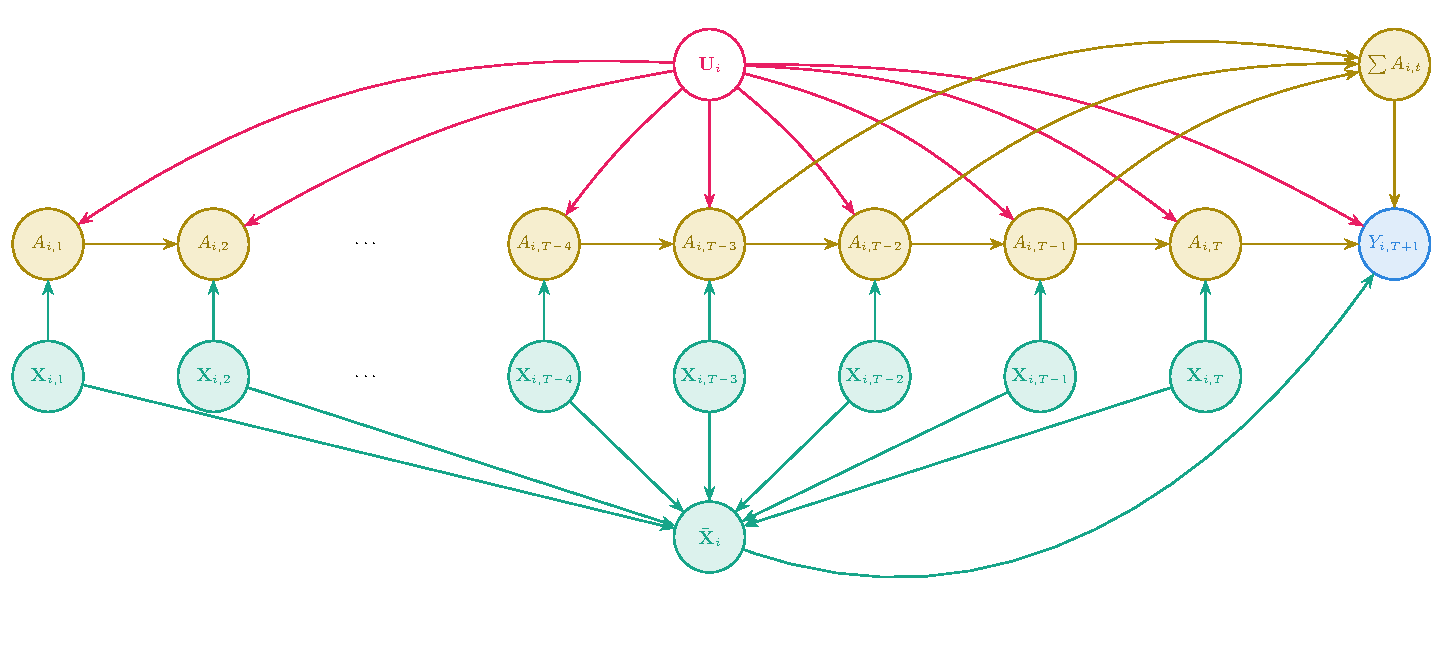
\includegraphics[width=\textwidth]{figures/build/dgp_dag.pdf}
    \caption{Data generating process causal DAG.}
    \label{fig:dgp-dag}
\end{figure}

\section{Estimation}
\label{estimation}
For defining our causal targets, first we need to specify the 
causal questions of interest. 
Define 
$$S_K(\underbar{a}_{T-K}) := \sum_{t=T-K}^{T-1} a_t 
\in \{0,1,2,\dots, K\}$$ 
as the sum 
of treatments received in the last $K$ time points before $T$, where $K+1$ 
represents the intervention window.  In real world applications, 
the choice of $K$ is based on the research question and the domain 
knowledge about the relevant time window for the treatment effects. 
In this simulation, we set $K=3$ to match the dependence structure of the 
outcome on the treatments in the DGP.

We are interested in two causal questions.
What is the average effect of the treatment received at the 
final time on the 
final outcome while holding fixed the sum of the earlier 
treatments within the intervention window, marginlized over the natural 
values of the treatments this treatment window? 
Mathematically, 
this is defined as
$\mathbb{E}\left[ Y_{iT}\left(a_T = 1, S_3 = s)\right) 
- Y_{iT}\left(a_T = 0, S_3 = s\right) \right]$. 
The second causal question is: what is the
average effect of receiving one additional treatment in 
the last three time points, 
before $T$ on the final outcome while keeping the final treatment 
fixed, marginalized over the natural 
values of the treatments in this window? To express 
this mathematically, we can write it as
$\mathbb{E}\left[Y_{iT}\left({S_3 = s, 
A_{iT} = a}\right) - Y_{iT}\left({S_3 = s+1, 
A_{iT} = a}\right)\right]$. 

To answer both of these causal questions, a marginal structural 
model is proposed  
that relates the assigned treatments to the expected potential 
outcome at the final time: 
$\mathbb{E\left[Y_{iT}\left(\underbar{a}_{T-k}\right)\right]} = 
g(\underbar{a}_{T-k}, \gamma_0)$, where 
$g(\underbar{a}_{T-k}, \gamma_0)$ is the true unkown function 
parameterized by $\gamma_0$. Our job is 
to first propose a function $f(\underbar{a}_{T-k}, \gamma)$ 
and then estimate its parameters $\gamma$. In this 
DGP, the ground truth function $g$, is: 
\begin{equation}
    \label{eq:truemsm}
    g\left(\underline{a}_{T-k}; \gamma_0 \right) = \alpha_0 + \tau_{F} a_T + \tau_{C} \sum_{t=T-3}^{T-1} a_t
\end{equation}

to see this, we begin from Eq.~\eqref{eq:blackwell_scm_outcome}. First note that since this is 
a sctructural equation model, we can replace the random variables 
by their interventional values. So we have:
\[
Y_{iT}\!\left(\underbar{a}_{T-k}\right)
= U_i + \tau_F a_T + \tau_C \sum_{t=T-3}^{T-1} a_t + \gamma^\top \bar X_{iT}(\underbar{a}_{T-k}) + \epsilon_{iT}.
\]
Taking the expectation on both sides and making use of 
the exogeneity of the covariates and treatments, we have:
\begin{align}
\label{eq:truemsmproof}
\mathbb{E}\!\left[Y_{iT}\!\left(\underbar{a}_{T-k}\right)\right]
&= \mathbb{E}[U_i] + \tau_F a_T + \tau_C \sum_{t=T-3}^{T-1} a_t
   + \gamma^\top \mathbb{E}[\bar X_{iT}] + \mathbb{E}[\epsilon_{iT}] \\
&= \mathbb{E}\!\left[U_i + \gamma^\top \bar X_{iT}\right]
   + \tau_F a_T + \tau_C \sum_{t=T-3}^{T-1} a_t \\
&= \alpha_0 + \tau_F a_T + \tau_C \sum_{t=T-3}^{T-1} a_t,
\qquad
\alpha_0 := \mathbb{E}\!\left[U_i + \gamma^\top \bar X_{iT}\right]
\end{align}
 
From Eq.~\eqref{eq:truemsm}, it can be seen: 

\begin{align*}
        &\mathbb{E}\left[ Y_{iT}\left(a_T = 1, S_3 = s\right) - Y_{iT}\left(a_T = 0, S_3 = s\right) \right] = \tau_F\\
        &\mathbb{E}\left[ Y_{iT}\left(a_T = a, S_3 = s+1\right) - Y_{iT}\left(a_T = a, S_3 = s\right) \right] = \tau_C
\end{align*}
The equality between these causal effects and the parameters of the 
outcome model in the DGP is a result of the linearity of the DGP and 
the absence of treatment-confounder feedback. 
See \ref{sec:msm_ground_truth} for more discussion on this. To only focus 
on the adjustment for the unmeasred confounder, for both of the methods, 
we specify $f\left(\underline{a}_{T-k}; \gamma \right)$ as the correctly 
specified linear MSM:
\begin{equation}
    f\left(\underline{a}_{T-k}; \gamma \right) = \alpha' + \tau_F' a_T + \tau_C' \sum_{t=T-3}^{T-1} a_t
\end{equation}
where $\gamma = (\alpha', \tau_F', \tau_C')$. 






 
 



